\documentclass[letterpaper]{article}

\usepackage[english]{babel}
\usepackage{amsmath}
\usepackage{amssymb}
\usepackage{amsthm}
\usepackage{booktabs}
\usepackage{csquotes}
\usepackage{float}
\usepackage{graphicx}
\usepackage{hyperref}
\usepackage{listings}
\usepackage{parskip}
\usepackage{tikz}
\usepackage[backend=biber,style=numeric]{biblatex}

\addbibresource{refs.bib}
\graphicspath{{imgs/}}

\newtheorem{theorem}{Theorem}
\newtheorem{lemma}{Lemma}

\newcommand{\RR}{\mathbb{R}}
\newcommand{\ZZ}{\mathbb{Z}}
\newcommand{\roots}{Z_{\RR}}
\newcommand{\sep}{\mathrm{sep}}
\newcommand{\size}{\mathrm{size}}
\newcommand{\bitsize}{\operatorname{bitsize}}
\newcommand{\citecorollary}[2][]{Corollary~#1 of~\cite{#2}}

\lstset{
  basicstyle=\ttfamily\small,
  columns=fullflexible,
  keepspaces=true,
  showstringspaces=false,
  frame=single,
  breaklines=true
}

\title{Real Root Isolation for Univariate Integer Polynomials}
\author{Mohamed BEN EL MOSTAPHA \\
Tom LLINARES UBERTALLI}
\date{January 2026}

\begin{document}

\maketitle

\begin{abstract}
This report studies the isolation of real roots of univariate polynomials with
integer coefficients. The implemented method is a subdivision algorithm based
on Descartes' rule of signs, Cauchy bounds, and rational changes of variables.
We describe the mathematical transformations used to reduce the problem to
positive-root counting, give a termination argument, and discuss the cost of
the dominant polynomial operations. The implementation relies on the FLINT
library for exact integer polynomial arithmetic. We also evaluate two
parallelization strategies and observe experimentally that, for high-degree
inputs, using FLINT's internal multithreading is more effective than exposing
parallelism only through the recursive subdivision tree.
\end{abstract}

\tableofcontents

\section{Introduction}

Let
\[
  f(x) = \sum_{i=0}^{d} a_i x^i \in \ZZ[x], \qquad a_d \neq 0,
\]
be a univariate integer polynomial. The real root isolation problem consists
in computing a finite family of rational intervals such that each real root of
$f$ lies in exactly one interval and each interval contains exactly one real
root. This is a fundamental subroutine in computer algebra: it is used before
root refinement, sign determination, quantifier elimination, and algorithms for
real algebraic numbers.

The project focuses on a subdivision algorithm. Instead of computing the roots
numerically, the algorithm recursively transforms intervals to the positive
real axis and applies Descartes' rule of signs. If the transformed polynomial
has no sign variation, the interval contains no positive root. If it has one
sign variation, the interval isolates one root. Otherwise the interval is
bisected and the same test is applied recursively.

The implementation is written in C and uses FLINT for exact polynomial
arithmetic. This is important because the intermediate coefficients can grow
quickly after repeated Taylor shifts and scaling transformations. A significant
part of the implementation effort therefore concerns both the mathematical
correctness of the transformations and the practical cost of the underlying
library operations.

The source code is available at
\href{https://github.com/Blurr327/real-root-isolation}
{\texttt{github.com/Blurr327/real-root-isolation}}.

\section{Notation and Problem Statement}

We work with a univariate polynomial
\[
  f(x)=a_d x^d+a_{d-1}x^{d-1}+\cdots+a_0 \in \ZZ[x],
  \qquad a_d \neq 0.
\]
The word ``univariate'' is important: there is only one unknown, $x$. This
makes it possible to use order on the real line and to represent the answer by
intervals. The coefficients are exact integers, so the algorithm must avoid
floating-point decisions that could become incorrect when two roots are very
close. We keep the notation $d$ for the degree and $\tau$ for the maximum
coefficient bitsize, as introduced in the previous section.

A complex number $\alpha$ is a root of multiplicity $m$ if
\[
  f(x)=(x-\alpha)^m g(x)
  \quad\text{with}\quad g(\alpha)\neq 0.
\]
Equivalently, $m$ is the largest exponent such that $(x-\alpha)^m$ divides
$f$ in $\mathbb{C}[x]$. In the square-free case every root has multiplicity
one. The implementation mainly targets square-free inputs, or inputs that have
first been reduced to square-free factors.

We denote the set of real roots by
\[
  \roots(f)=\{\alpha\in\RR \mid f(\alpha)=0\}.
\]
When $f$ has at least two distinct real roots, its real-root separation is
\[
  \sep(f)=
  \min_{\substack{\alpha,\beta\in\roots(f)\\ \alpha\neq\beta}}
  |\alpha-\beta|.
\]
This quantity matters because it controls how narrow isolating intervals may
need to become. If two roots are extremely close, any correct algorithm must
eventually produce endpoints precise enough to separate them.

The subdivision algorithm also uses the number of sign variations. If
\[
  f(x)=\sum_{i=0}^{d}a_i x^i,
\]
let $i_0<i_1<\cdots<i_r$ be the indices for which $a_{i_j}\neq 0$. Then
\[
  V(f)=
  \#\left\{
    0\leq j<r \mid
    \operatorname{sign}(a_{i_j})\operatorname{sign}(a_{i_{j+1}})=-1
  \right\}.
\]
In words, zero coefficients are ignored, and $V(f)$ counts how many times the
remaining coefficient signs switch from positive to negative or from negative
to positive. Finally, $Z_{>0}(f)$ denotes the number of strictly positive real
roots of $f$, counted with multiplicity.

The goal is to compute a finite ordered family of rational intervals
\[
  S=\{[a_1,b_1],\ldots,[a_s,b_s]\},
  \qquad a_i,b_i\in\mathbb{Q},
\]
such that
\[
  a_i\leq b_i < a_{i+1}\leq b_{i+1}
  \quad\text{for every } 1\leq i<s,
\]
and
\[
  \forall i,\quad |[a_i,b_i]\cap\roots(f)|=1,
  \qquad
  \roots(f)\subseteq \bigcup_{i=1}^{s}[a_i,b_i].
\]
The strict inequality $b_i<a_{i+1}$ explicitly forbids overlapping intervals.
Intervals of the form $[a_i,a_i]$ are allowed; they represent roots that are
found exactly during the computation.

Several families of algorithms solve this problem. Sturm-based methods use a
Sturm sequence to count roots exactly in an interval. Descartes methods, such
as the one implemented in this project, use changes of variables and
Descartes' rule of signs to discard or isolate intervals
\cite{collinsAkritas1976,rouillierZimmermann2004}. Continued-fraction methods
form another important family and are closely related to Descartes
subdivision. In practice, computer algebra systems and libraries combine these
mathematical ideas with optimized exact arithmetic; in this project, the
low-level integer polynomial operations are delegated to FLINT \cite{flint}.

\section{Input and Output Size: A Complexity Baseline}

Before designing an algorithm, it is useful to ask what complexity one can
reasonably hope for. A root isolation algorithm cannot be faster than the time
needed to read its input, and it also cannot be faster than the time needed to
write its output. Thus, the input and output sizes give a first lower bound on
the best possible complexity.

For an integer $a\neq 0$, let
\[
  \bitsize(a)=\lfloor \log_2 |a| \rfloor + 1,
\]
and set $\bitsize(0)=1$. If
\[
  f(x)=\sum_{i=0}^{d}a_i x^i \in \ZZ[x],
\]
we define
\[
  \tau=\tau(f)=\max_{0\leq i\leq d}\bitsize(a_i).
\]
In the dense representation used in this project, the input consists of
$d+1$ integer coefficients, each of size at most $\tau$. Therefore the input
size is
\[
  \size_{\mathrm{in}}(f)=O(d\tau).
\]

The output size is controlled by root separation. Let
\[
  \sep(f)=
  \min_{\substack{\alpha,\beta\in\roots(f)\\ \alpha\neq\beta}}
  |\alpha-\beta|
\]
be the minimum distance between two distinct real roots. Classical separation
bounds for integer polynomials, such as \citecorollary[10.22]{basuPollackRoy2006},
give a lower bound
\[
  \sep(f)
  \geq
  \left(\frac{d}{\sqrt{3}}\right)^{-1}
  d^{-d/2}
  (d+1)^{(1-d)/2}
  2^{\tau(1-d)}.
\]
We denote this lower bound by
\[
  \phi(d,\tau)
  =
  \left(\frac{d}{\sqrt{3}}\right)^{-1}
  d^{-d/2}
  (d+1)^{(1-d)/2}
  2^{\tau(1-d)}.
\]
For the complexity discussion, the exact constants are less important than the
order of magnitude:
\[
  \phi(d,\tau)=2^{-O(d\tau+d\log d)}.
\]
Thus the number of bits needed to resolve the worst-case separation is
\[
  \log_2\!\left(\frac{1}{\phi(d,\tau)}\right)
  =O(d\tau+d\log d).
\]

This explains the target size of the isolating intervals. If the output
intervals are ordered
\[
  [a_1,b_1], [a_2,b_2], \ldots, [a_s,b_s],
\]
and each interval is refined until
\[
  b_i-a_i \leq \phi(d,\tau),
\]
then an interval cannot contain two distinct real roots: two such roots would
be closer than the guaranteed separation bound. In practice one may use a
constant factor such as $\phi(d,\tau)/2$, but this does not change the
asymptotic number of bits required for the endpoints.

Since a degree-$d$ polynomial has at most $d$ real roots, the output contains
at most $d$ intervals. Each endpoint may require
$O(d\tau+d\log d)$ bits in the worst case. Hence the total output size is of
order
\[
  \size_{\mathrm{out}}(f)
  =O\!\left(d(d\tau+d\log d)\right)
  =O(d^2\tau+d^2\log d).
\]

Combining input and output, even an ideal root isolation algorithm should not
be expected to have complexity below
\[
  \Omega\!\left(d\tau+d^2\tau+d^2\log d\right)
\]
in the worst case when the full isolating family is written explicitly. This
does not prove that our subdivision algorithm reaches this bound, but it gives
a benchmark: the closer the implementation comes to being polynomial in the
input size plus the unavoidable output size, the better the algorithmic
behavior we can hope for.

\section{Mathematical Background}

\subsection{Descartes' Rule of Signs}

\begin{theorem}[Descartes' rule of signs]
Let $f \in \RR[x]$. The number $Z_{>0}(f)$ of strictly positive real roots of
$f$, counted with multiplicity, is at most $V(f)$. Moreover,
$V(f)-Z_{>0}(f)$ is even.
\end{theorem}

\begin{proof}
We first prove the parity statement. Assume, without loss of generality, that
the constant coefficient is non-zero; otherwise one may divide by the largest
power of $x$ dividing $f$, which does not change the number of strictly
positive roots. The number of sign variations in the coefficient sequence is
even exactly when the first and last non-zero coefficients have the same sign,
and it is odd exactly when they have opposite signs. Equivalently, $V(f)$
records whether the signs of $f(0)$ and $f(x)$ for $x$ sufficiently large and
positive agree or disagree.

On the other hand, when $x$ moves from $0$ to $+\infty$, the sign of $f(x)$
changes exactly at positive roots of odd multiplicity. Roots of even
multiplicity touch the axis without changing sign. Therefore the parity of the
number of positive roots counted with multiplicity is also determined by
whether the signs at $0$ and $+\infty$ agree. Hence
\[
  Z_{>0}(f)\equiv V(f)\pmod 2.
\]

It remains to prove the inequality $Z_{>0}(f)\leq V(f)$. We proceed by
induction on the degree. The result is clear for constant polynomials. Let
$f$ have degree $d\geq 1$, and assume the result for polynomials of smaller
degree. Suppose that $f$ has $r$ distinct positive roots, with multiplicities
$m_1,\ldots,m_r$. Then
\[
  Z_{>0}(f)=m_1+\cdots+m_r.
\]
The derivative $f'$ has each of these roots with multiplicity one less, and
Rolle's theorem gives at least one additional root of $f'$ between every two
consecutive distinct positive roots of $f$. Thus
\[
  Z_{>0}(f')\geq
  (m_1-1)+\cdots+(m_r-1)+(r-1)
  =
  Z_{>0}(f)-1.
\]
By the induction hypothesis,
\[
  Z_{>0}(f')\leq V(f').
\]
The coefficient sequence of $f'$ is obtained from that of $f$ by deleting the
constant term and multiplying the remaining coefficients by positive
integers, so the signs among the remaining coefficients do not change.
Deleting the first coefficient can remove at most one sign variation, hence
\[
  V(f')\leq V(f).
\]
Combining these inequalities gives
\[
  Z_{>0}(f)\leq Z_{>0}(f')+1\leq V(f')+1\leq V(f)+1.
\]
Since $Z_{>0}(f)$ and $V(f)$ have the same parity, the case
$Z_{>0}(f)=V(f)+1$ is impossible. Therefore $Z_{>0}(f)\leq V(f)$.
\end{proof}

The algorithm uses the following consequences. If $V(f)=0$, then $f$ has no
strictly positive real root. If $V(f)=1$, then $f$ has exactly one strictly
positive real root. If $V(f) \geq 2$, the test is inconclusive and the
corresponding interval must be subdivided.

\subsection{Cauchy Bound}

Before subdivision, the algorithm bounds the search domain. If
\[
  f(x)=a_d x^d + a_{d-1}x^{d-1} + \cdots + a_0,
  \qquad a_d \neq 0,
\]
then every complex root $\alpha$ of $f$ satisfies the Cauchy bound
\[
  |\alpha| \leq 1 + \max_{0 \leq i < d} \left|\frac{a_i}{a_d}\right|.
\]

\begin{proof}
Let
\[
  H=\max_{0\leq i<d}\left|\frac{a_i}{a_d}\right|.
\]
If $|\alpha|\leq 1$, then the bound is immediate. Assume therefore that
$|\alpha|>1$. Since $f(\alpha)=0$, we have
\[
  a_d\alpha^d=-\sum_{i=0}^{d-1}a_i\alpha^i.
\]
Taking absolute values and dividing by $|a_d|$ gives
\[
  |\alpha|^d
  \leq
  \sum_{i=0}^{d-1}\left|\frac{a_i}{a_d}\right||\alpha|^i
  \leq
  H\sum_{i=0}^{d-1}|\alpha|^i.
\]
Because $|\alpha|>1$,
\[
  \sum_{i=0}^{d-1}|\alpha|^i
  =
  \frac{|\alpha|^d-1}{|\alpha|-1}
  <
  \frac{|\alpha|^d}{|\alpha|-1}.
\]
Thus
\[
  |\alpha|^d
  <
  H\frac{|\alpha|^d}{|\alpha|-1}.
\]
After cancelling $|\alpha|^d>0$, we obtain $|\alpha|-1<H$, and therefore
\[
  |\alpha|<1+H.
\]
The non-strict bound follows immediately.
\end{proof}

The implementation rounds this bound upward to a power of two, $2^b$. This
choice makes the subsequent scaling operation efficient because multiplying by
powers of two corresponds to bit shifts on integer coefficients.

\section{Subdivision Algorithm}

\subsection{Changes of Variables}

The algorithm repeatedly reduces root isolation on an interval to positive
root counting. Three transformations are used.

\paragraph{Scaling to the unit interval.}
After computing a bound $B=2^b$, positive roots in $(0,B)$ are mapped to
$(0,1)$ by the substitution
\[
  x = B y.
\]
For integer polynomials and powers of two, the transformed polynomial can be
represented with integer coefficients using coefficient shifts.

\paragraph{Mapping the unit interval to positive roots.}
To test whether an interval contains roots, roots in $(0,1)$ are mapped to
$(0,+\infty)$ using
\[
  x = \frac{1}{y+1}.
\]
If $f$ has degree $d$, the transformed polynomial is
\[
  g(y) = (y+1)^d f\!\left(\frac{1}{y+1}\right).
\]
Computationally, this is obtained by reversing the coefficients of $f$ and
then applying a Taylor shift by $1$. Descartes' rule is then applied to $g$.

\paragraph{Bisection.}
If the sign variation test is inconclusive, the current interval is split into
two halves. On the normalized interval $(0,1)$, the two substitutions are
\[
  x = \frac{y}{2}
  \qquad\text{and}\qquad
  x = \frac{y+1}{2}.
\]
The first maps the left half to $(0,1)$ and the second maps the right half to
$(0,1)$.

\subsection{Algorithm Description}

The core recursive procedure receives a polynomial whose roots of interest
have already been mapped into the current interval. It applies the
$(0,1)\rightarrow(0,+\infty)$ transformation, counts sign variations, and
either rejects the interval, accepts it as isolating, or subdivides it.

\begin{lstlisting}
subdivide(poly, start, end):
    transformed = reverse(poly)
    transformed = taylor_shift(transformed, 1)
    variations = count_sign_variations(transformed)

    if variations == 0:
        return

    if variations == 1:
        output [start, end]
        return

    mid = (start + end) / 2

    left_poly = substitute(poly, x = y / 2)
    left_parity = subdivide(left_poly, start, mid)

    right_poly = substitute(poly, x = (y + 1) / 2)
    right_parity = subdivide(right_poly, mid, end)

    if (left_parity + right_parity) mod 2 != variations mod 2:
        output [mid, mid]

    return variations mod 2
\end{lstlisting}

The complete algorithm runs this procedure twice: once for positive roots, and
once after the change of variable $x \mapsto -x$ for negative roots.

An important detail of the sequential implementation is the way it detects
whether the midpoint is itself a root. A direct approach would evaluate the
original polynomial at the midpoint after every split. Instead, the sequential
code uses the parity statement in Descartes' rule. The parent interval has a
variation count $c$, while the left and right recursive calls return the
parities $c_1$ and $c_2$ of their variation counts. If the midpoint is not a
root, the roots of the parent interval are exactly the roots of the two open
children, so the parities agree:
\[
  c \equiv c_1+c_2 \pmod 2.
\]
If this congruence fails, the missing root must be the boundary point between
the two children, so the algorithm adds the exact interval $[\mathrm{mid},
\mathrm{mid}]$. This avoids an extra exact polynomial evaluation in the
sequential version.

The parallel implementation does not use this optimization. In the OpenMP task
version, the two recursive calls are launched as tasks whose main purpose is
to append intervals to the shared output vector. In practice, relying on the
tasks to return the exact parity information was unreliable: depending on the
task structure and synchronization, the value available to the parent could be
missing or could correspond to the wrong recursive branch. To avoid adding
incorrect midpoint roots, the parallel version uses the safer direct test
$f(\mathrm{mid})=0$ instead. This costs an extra exact evaluation, but it keeps
the parallel algorithm correct.

\section{Termination and Correctness}

We assume in this section that $f$ is square-free. Multiple roots can be
handled separately by a square-free factorization step. We also assume that
roots lying exactly on endpoints are detected and recorded separately, so the
recursive test is applied to open intervals.

Let
\[
  I=(c,c+w)
\]
be an interval examined by the subdivision algorithm. To count roots in this
interval, the algorithm uses the Mobius transformation
\[
  x = c+\frac{w}{y+1}.
\]
Positive values of $y$ are mapped exactly to points of $I$. After clearing
denominators, we obtain the polynomial
\[
  Q(y)=(y+1)^d f\!\left(c+\frac{w}{y+1}\right).
\]
The positive roots of $Q$ correspond to the roots of $f$ in $I$, and
Descartes' rule gives an upper bound through the number of sign variations
$V(Q)$.

The key point for termination is the geometry of this transformation. The
inverse change of variable maps the right half-plane
\[
  \operatorname{Re}(y)>0
\]
to the open disk $D(I)$ whose diameter is the interval $I$. Equivalently,
$D(I)$ is centered at $c+w/2$ and has radius $w/2$. This disk interpretation
is the standard geometric view behind Descartes subdivision methods and is
closely related to Obreschkoff's theorem
\cite{collinsAkritas1976,rouillierZimmermann2004}.

In the form needed here, the theorem says that if the disk $D(I)$ and its
boundary contain no roots of $f$, then the transformed polynomial has no sign
variation. If the disk contains exactly one simple real root and no other root
lies in the disk or on its boundary, then the transformed polynomial has one
sign variation. Thus, once intervals are small enough that their associated
disks isolate either zero roots or one simple real root, Descartes' test stops
the recursion.

It remains to justify that this situation is eventually reached. Since $f$ is
square-free, it has finitely many distinct roots. Let
\[
  \Delta =
  \min_{\alpha\neq\beta,\ f(\alpha)=f(\beta)=0}
  |\alpha-\beta|
\]
be the minimum distance between two distinct complex roots. If all roots are
real this is already enough. If non-real roots occur, define also
\[
  \delta =
  \min\{|\operatorname{Im}(z)| \mid f(z)=0,\ z\notin\RR\}.
\]
When there are no non-real roots, this second quantity is not needed. In all
cases, the relevant quantities are strictly positive because the set of roots
is finite and $f$ is square-free.

Now consider a branch at depth $h$. Its interval width is
\[
  w_h = \frac{w_0}{2^h},
\]
where $w_0$ is the width of the initial bounded interval. As $h$ grows,
$w_h$ tends to zero. Hence eventually $w_h<\Delta$. At that point the disk
with diameter $I$ is too small to contain two distinct roots. Also, if
non-real roots exist and $w_h<2\delta$, then the radius $w_h/2$ is smaller
than the distance of every non-real root from the real axis. Therefore no
non-real root can lie in such a disk centered on the real axis.

For sufficiently large $h$, each interval is therefore in one of two cases:
\begin{itemize}
  \item its disk contains no root of $f$;
  \item its disk contains exactly one simple real root of $f$.
\end{itemize}
By the Obreschkoff/Descartes disk criterion cited above, these two cases give
$V(Q)=0$ and $V(Q)=1$, respectively. Both are stopping cases of the
algorithm. Consequently no branch can continue forever, and the subdivision
algorithm terminates.

Correctness follows from the same argument. If $V(Q)=0$, Descartes' rule
implies that the interval contains no real root. If $V(Q)=1$, Descartes' rule
and parity imply that the interval contains exactly one real root. The
recursive bisection covers the whole initial search domain, while Cauchy's
bound guarantees that all real roots lie in that domain. Running the procedure
for positive roots and then after $x\mapsto -x$ covers all real roots of $f$.

\section{Complexity of the Subdivision Algorithm}

The running time is governed by two simple questions:
\begin{itemize}
  \item how deep can the subdivision tree become?
  \item how expensive is one interval test?
\end{itemize}
The first question is controlled by root separation. The second one is
controlled by exact polynomial arithmetic, especially Taylor shifts.

\subsection{How Deep Can the Tree Become?}

The algorithm starts from a bounded interval $(-B,B)$, where $B$ is obtained
from Cauchy's root bound and rounded to a power of two. Since the input
coefficients have bitsize at most $\tau$, this initial bound has
\[
  \log_2 B = O(\tau).
\]

Every subdivision divides the interval length by two. After $h$ subdivisions,
the interval length is approximately $B/2^h$. In the worst case, subdivision
must continue until the intervals are smaller than the minimum distance
between two distinct real roots. Using the separation lower bound
\[
  \sep(f)\geq \phi(d,\tau),
\]
it is enough to reach
\[
  \frac{B}{2^h}\leq \phi(d,\tau).
\]
Therefore the required depth satisfies
\[
  h = O\!\left(\log_2 B+\log_2\!\left(\frac{1}{\phi(d,\tau)}\right)\right).
\]
From the bound on $\phi(d,\tau)$ established earlier,
\[
  \log_2\!\left(\frac{1}{\phi(d,\tau)}\right)
  = O(d\tau+d\log d).
\]
Thus a useful worst-case estimate for the maximum depth is
\[
  H = O(d\tau+d\log d).
\]

This is the most important theoretical estimate in the section. It says that
hard inputs are hard because roots can be very close, and close roots force
many bisections.

\subsection{What Does One Interval Test Cost?}

For each interval, the algorithm changes variables so that roots in the
interval become positive roots of a transformed polynomial. It then applies
Descartes' rule by counting sign variations.

The sign count itself is cheap: it scans the coefficient list once, so it is
linear in the degree. The expensive part is producing the transformed
polynomial. In the implementation this uses FLINT polynomial operations,
notably Taylor shifts. If $C_{\mathrm{shift}}(d,L)$ denotes the cost of a
Taylor shift for a degree-$d$ polynomial with coefficients of bitsize $L$,
then one interval test costs approximately
\[
  C_{\mathrm{shift}}(d,L).
\]
The additional sign-counting work is smaller and is not the bottleneck in the
experiments.

There is also an important practical issue: $L$ grows during the algorithm.
Changes of variables and Taylor shifts can make the coefficients much larger
than the original input coefficients. This means that deeper nodes are usually
more expensive than shallow nodes.

\subsection{Total Cost}

Let $N$ be the number of intervals actually tested by the algorithm. Then the
running time can be read as
\[
  \text{running time}
  \approx
  N \times \text{cost of one transformed interval test}.
\]
More explicitly, a reasonable summary is
\[
  T
  =
  O\!\left(N\cdot C_{\mathrm{shift}}(d,L)\right),
\]
where $L$ represents the coefficient sizes reached during the computation.

The value of $N$ depends strongly on the input polynomial. If Descartes' test
quickly returns $0$ or $1$, many branches stop early. If the test remains
inconclusive for many nearby roots, the algorithm explores deeper. A complete
binary tree of depth $H$ would have exponentially many nodes, but this is a
very pessimistic picture for root isolation: most intervals do not contain a
root, and intervals containing a single root eventually stop.

The intended behavior is therefore output-sensitive. Since there are at most
$d$ real roots and the needed endpoint precision is controlled by
$H=O(d\tau+d\log d)$, the natural target is to run in time polynomial in
the input size and in the output precision. The implementation does not prove
such an optimal bound, but the analysis identifies exactly where the time is
spent: in the number of visited intervals and in the cost of exact polynomial
transformations.

\section{Implementation}

The implementation is written in C. Integer polynomials, rational numbers, and
Taylor shifts are handled using FLINT. The main implemented components are:
\begin{itemize}
  \item computation of a Cauchy bound rounded to a power of two;
  \item coefficient scaling for substitutions of the form $x=2^k y$;
  \item sign variation counting;
  \item Taylor shifts using FLINT routines;
  \item recursive subdivision with exact rational endpoints;
  \item a parallel version using OpenMP tasks and FLINT threads.
\end{itemize}

Using a library such as FLINT avoids reimplementing highly optimized arithmetic
for large integer polynomials. This also makes the performance profile clearer:
the dominant cost is not sign variation counting, but the repeated exact
polynomial transformations, especially Taylor shifts.

\section{Experimental Observations}

\subsection{Experimental Setup}

All timings in this section were obtained on the same laptop used for
development. The machine has an Intel Core i5-6300U processor, with two
physical cores and two hardware threads per core. Thus, the operating system
exposes four logical CPUs, but only two of them are physical cores. This point
is important when interpreting the parallel results: using four software
threads on this machine means using simultaneous multithreading, not four
independent physical cores.

\begin{center}
\begin{tabular}{ll}
\toprule
Component & Specification \\
\midrule
CPU & Intel Core i5-6300U at 2.40 GHz \\
Physical cores & 2 \\
Logical CPUs & 4 \\
Maximum CPU frequency & 3.00 GHz \\
Memory & 7.2 GiB RAM \\
Operating system & Ubuntu 22.04, Linux kernel 6.8.0 \\
Compiler flags & \texttt{-O3 -march=native -fopenmp} \\
Arithmetic library & FLINT, linked with GMP \\
\bottomrule
\end{tabular}
\end{center}

The benchmark executable was built with
\[
  \texttt{make test\_parallel\_rri\_algo}.
\]
Unless otherwise stated, inputs are random square-free dense integer
polynomials generated by the test program.

\subsection{Taylor Shift Cost}

Taylor shifts are one of the most expensive operations in the algorithm. We
measured their cost on random integer polynomials while varying the degree and
the coefficient bitsize. The observed behavior is consistent with a strong
dependence on the degree and a roughly linear dependence on coefficient
bitsize for the tested range.

\begin{figure}[H]
  \centering
  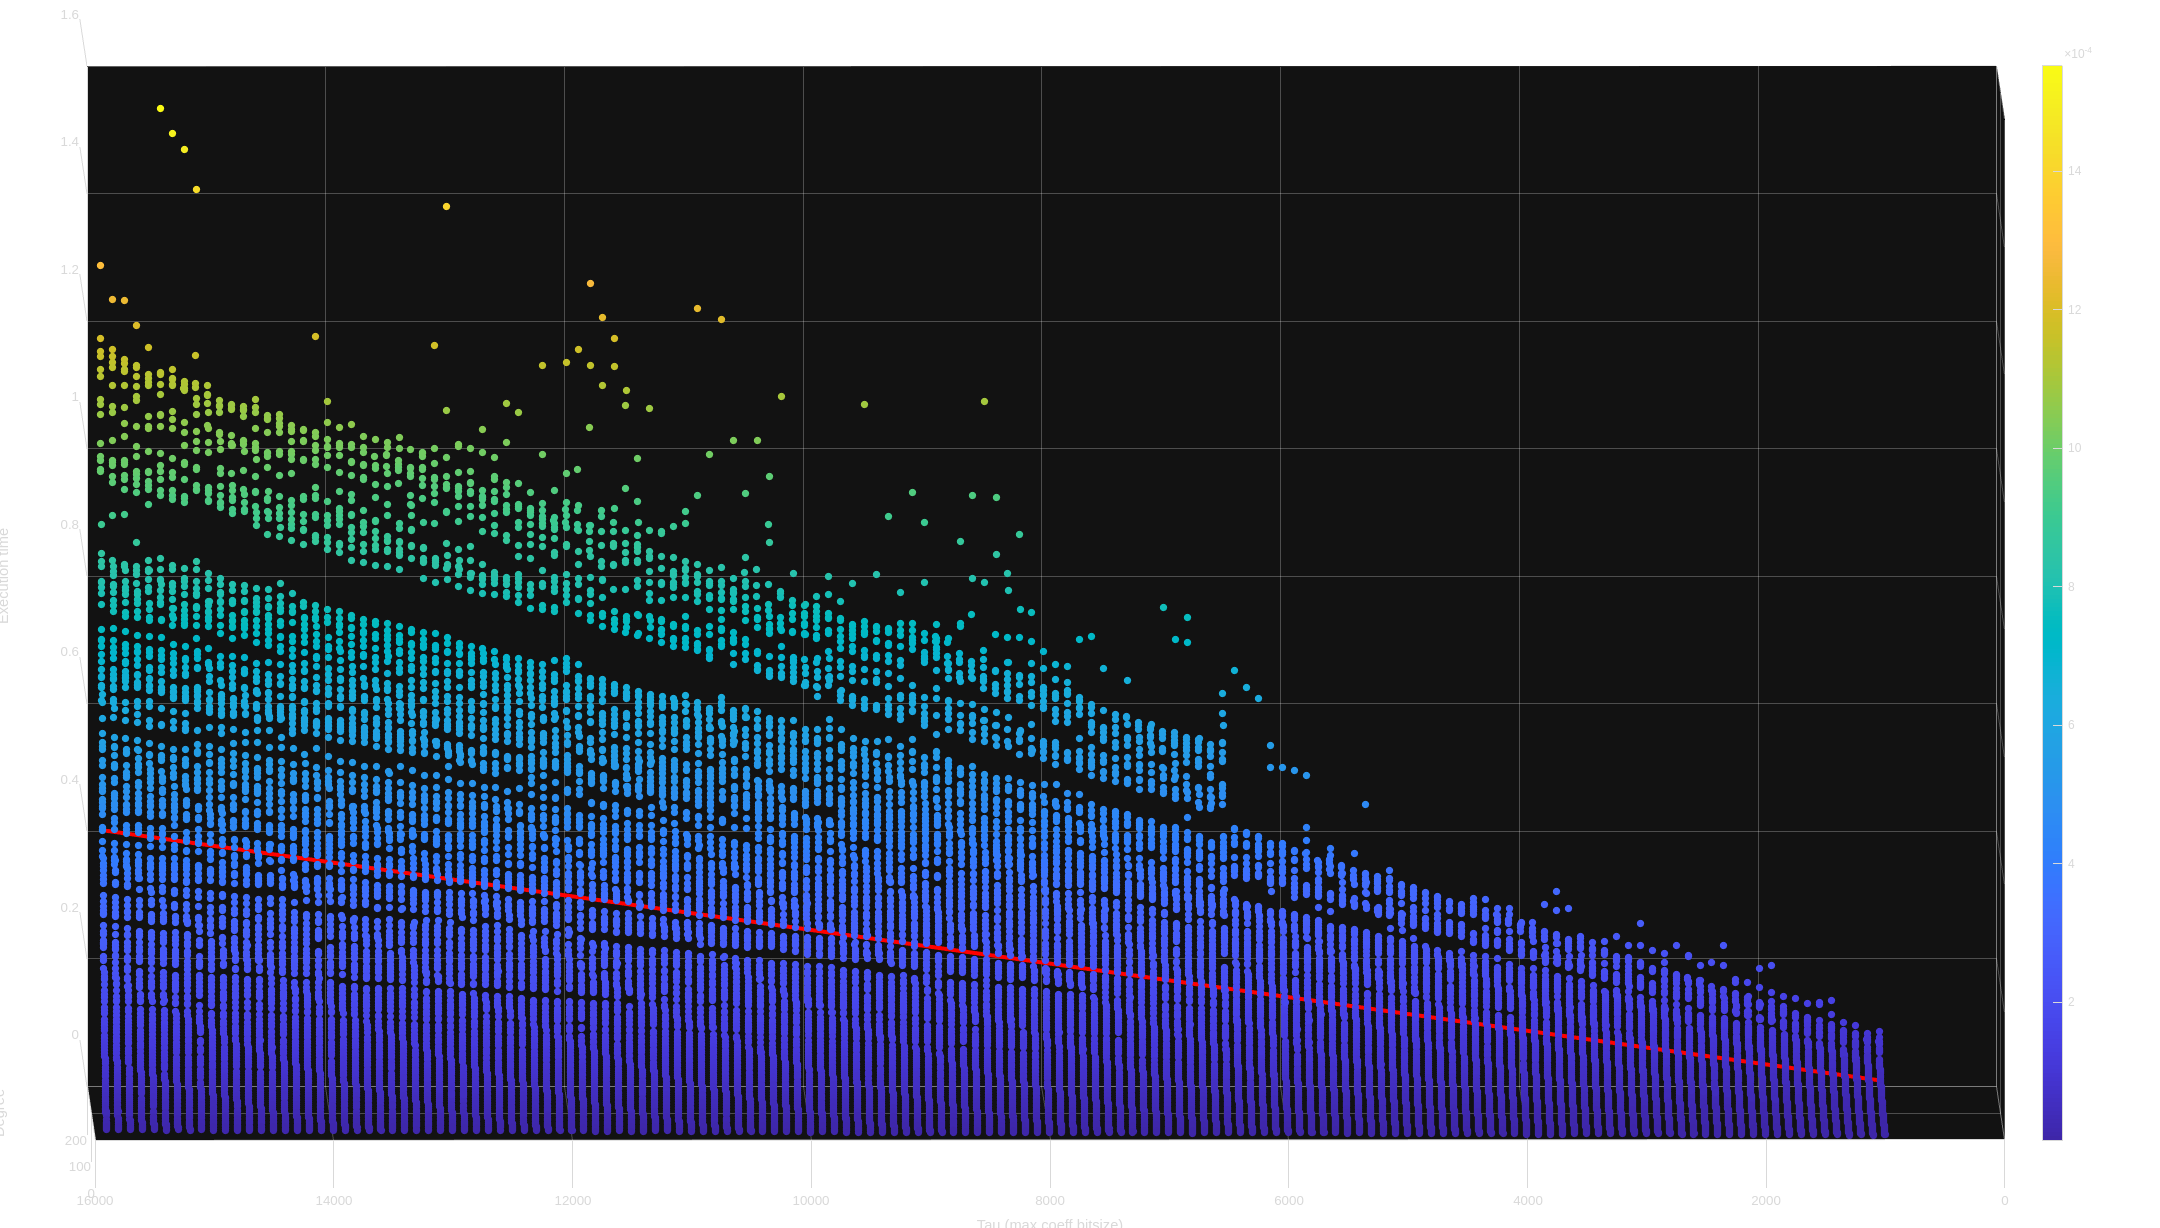
\includegraphics[width=0.65\textwidth]{taylor_shift complexity/taylor_shift_bitsize.png}
  \caption{Taylor shift running time with respect to coefficient bitsize.}
  \label{fig:taylorcoeff}
\end{figure}

\begin{figure}[H]
  \centering
  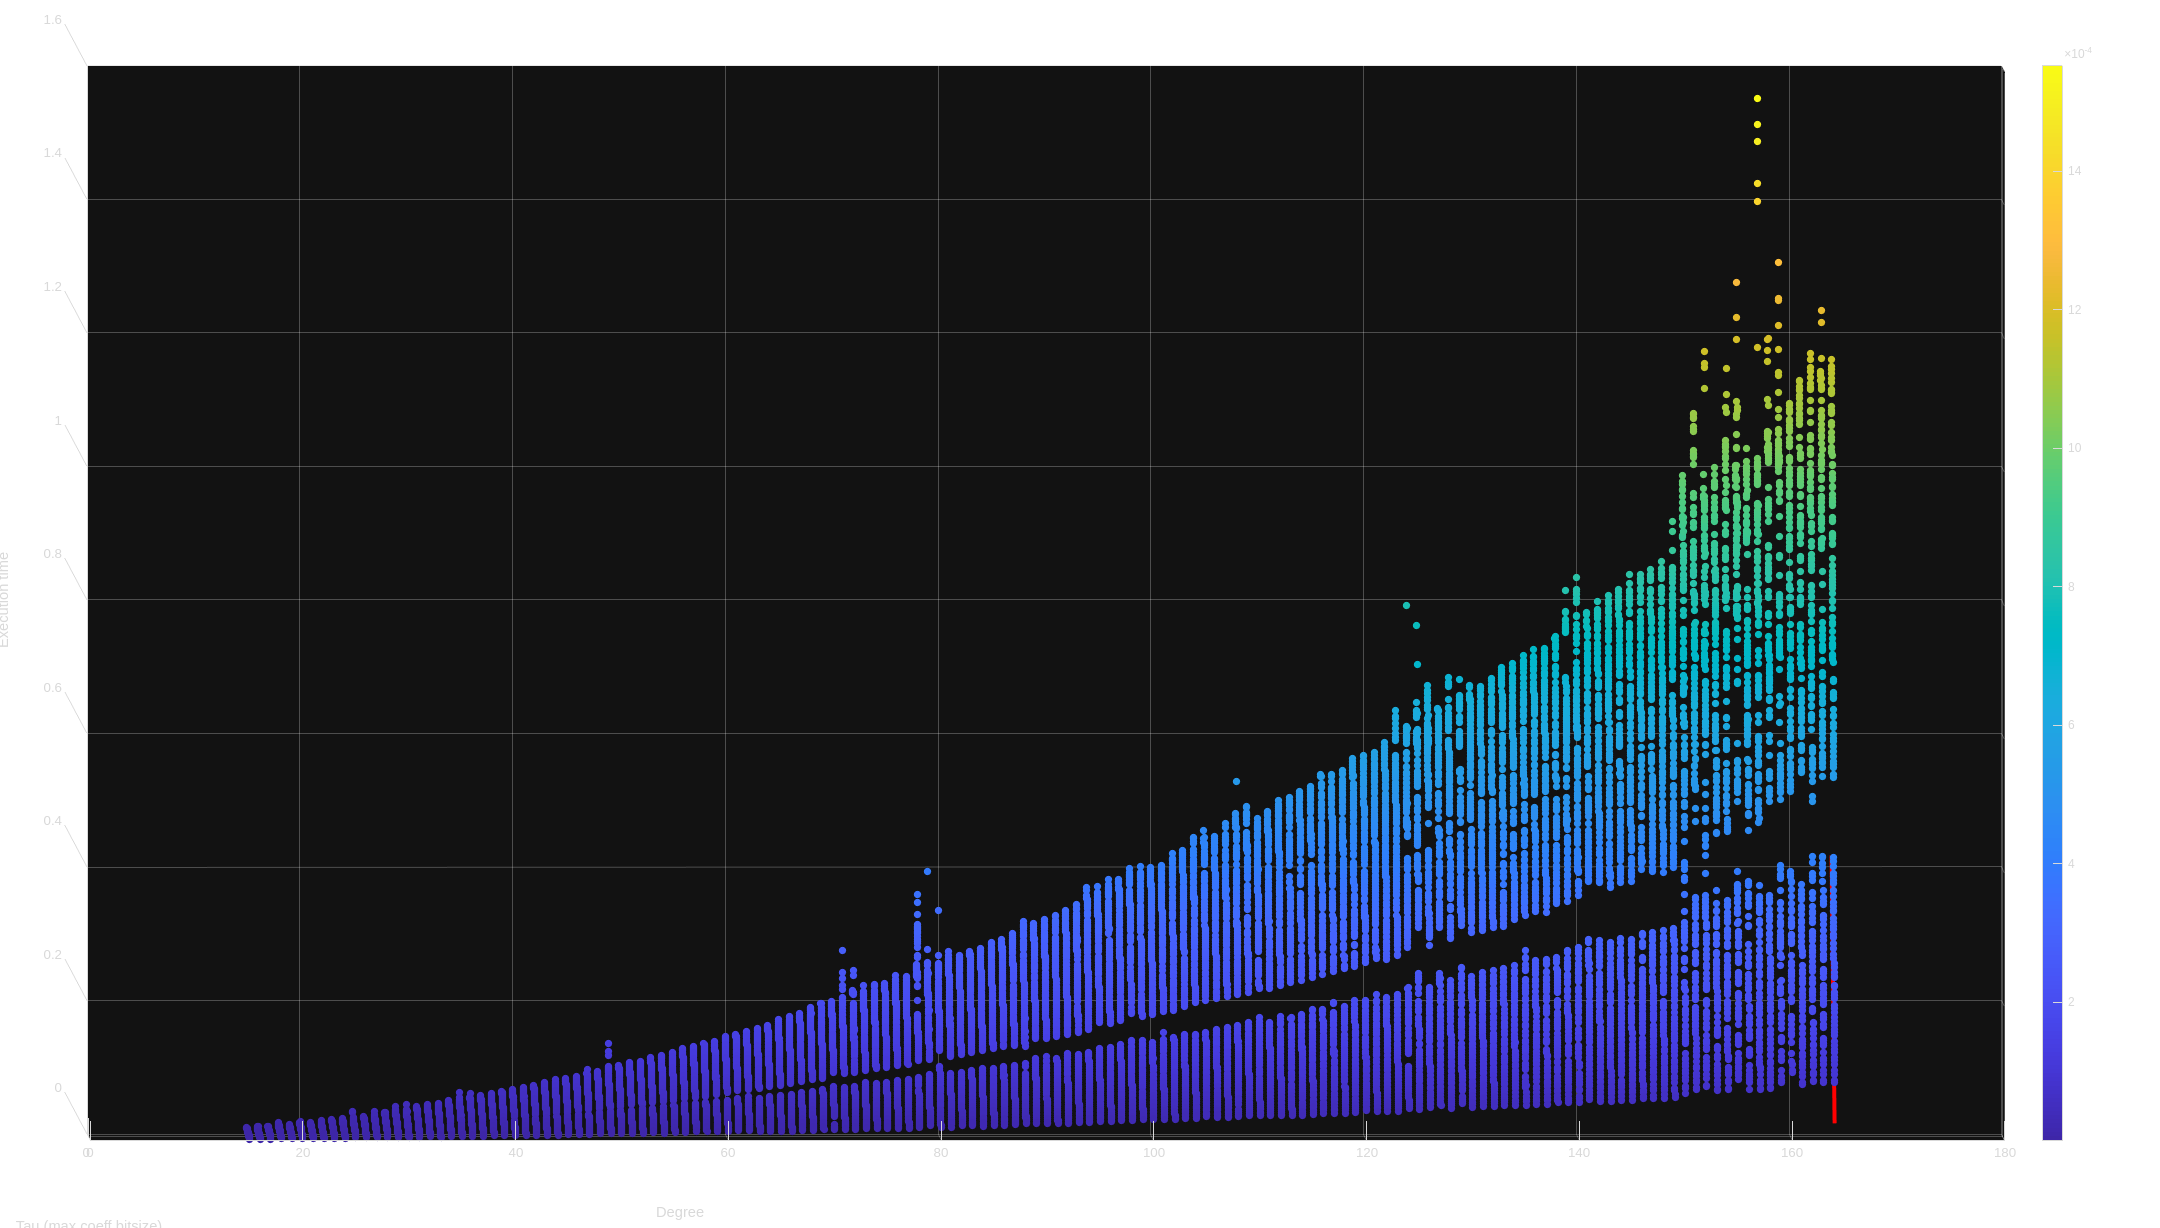
\includegraphics[width=0.65\textwidth]{taylor_shift complexity/taylor_shift_degree.png}
  \caption{Taylor shift running time with respect to polynomial degree.}
  \label{fig:taylordegree}
\end{figure}

\begin{figure}[H]
  \centering
  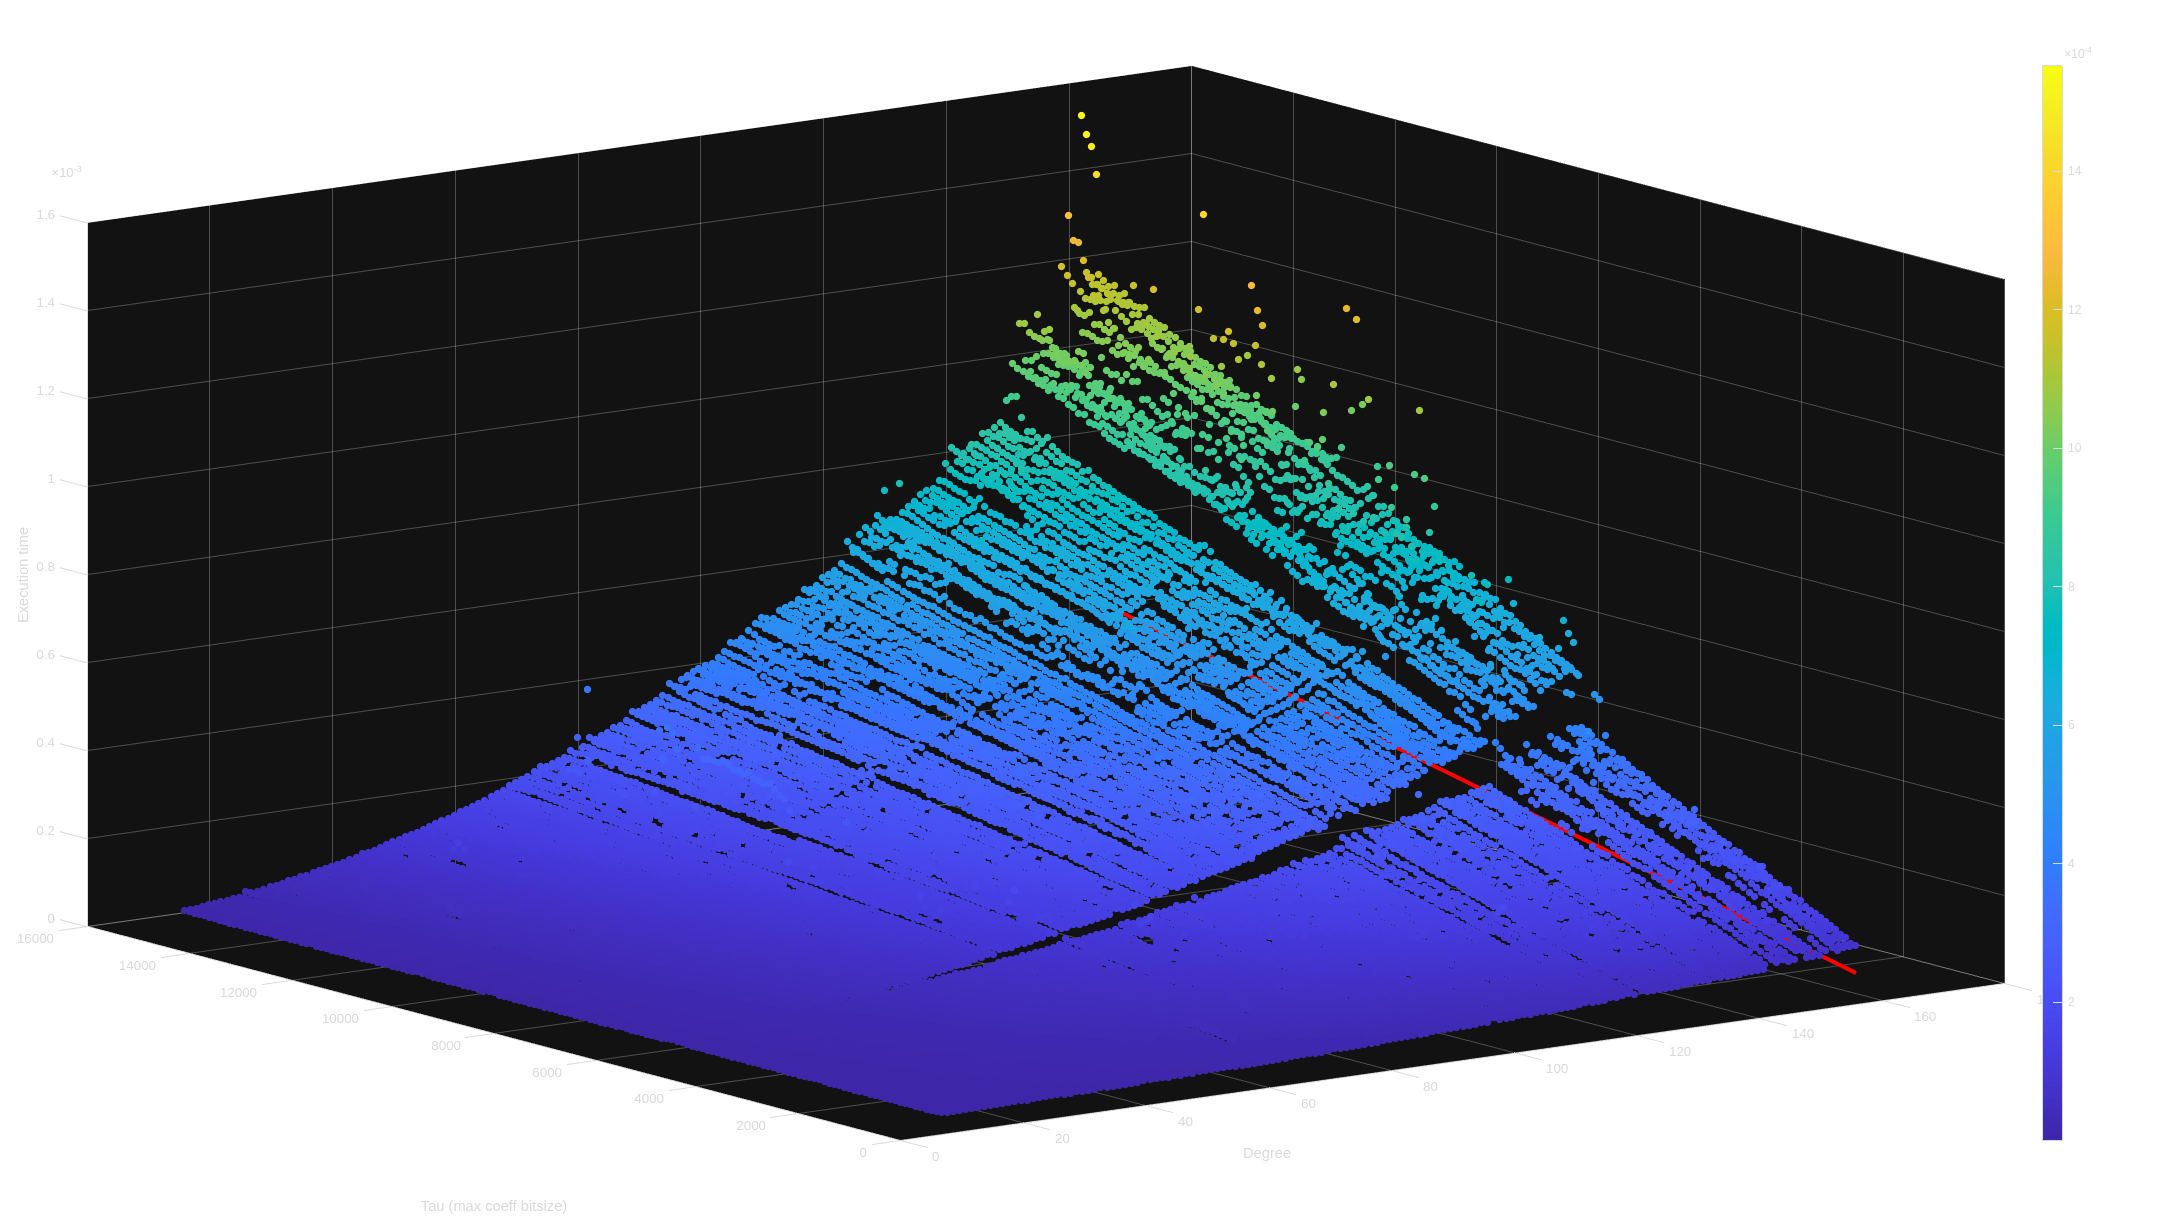
\includegraphics[width=0.65\textwidth]{taylor_shift complexity/taylor_shift_full.png}
  \caption{Taylor shift running time with respect to both degree and coefficient bitsize.}
  \label{fig:taylorfull}
\end{figure}

\subsection{Coefficient Growth}

The changes of variables can substantially increase coefficient sizes. In our
tests, Taylor shifts increased the largest coefficient by roughly 195 bits on
average for the selected parameter range. The scaling substitution
$x=2^b y$ can be even more aggressive: for degree $200$ and coefficient
bitsize $8$, the average increase was about $1600$ bits.

We also tested whether a large common factor could often be removed after the
scaling step. In the same setting, the average gcd of the transformed
coefficients was about $4.37$, which is too small to be a useful compression
strategy. This suggests that coefficient growth is a genuine computational
obstacle rather than an artifact that can usually be removed by normalization.

\subsection{Root Isolation Timings}

The following table summarizes representative outputs of the current
benchmark harness on random dense polynomials of degree $1000$ with
32-bit coefficients. Each row uses three random tests and reports the
individual running times printed by the program, followed by the average time.

\begin{center}
\small
\begin{tabular}{lllll}
\toprule
OMP & FLINT & Times (s) & Average (s) & Intervals \\
\midrule
1 & 1 & 1.799, 2.344, 0.823 & 1.655 & 6, 6, 4 \\
4 & 1 & 1.615, 0.263, 0.307 & 0.728 & 6, 2, 4 \\
2 & 2 & 1.562, 1.897, 2.686 & 2.048 & 8, 6, 6 \\
1 & 4 & 1.249, 0.350, 1.042 & 0.880 & 6, 2, 6 \\
\bottomrule
\end{tabular}
\end{center}

The tested commands had the following form:
\[
  \texttt{./test\_parallel\_rri\_algo --degree 1000 --bits 32 --tests 3}
\]
with the two thread parameters changed according to the table. All runs
successfully passed the interval verification step.

For a larger input, a representative run on a random polynomial of degree
$5000$ with 32-bit coefficients gave the following performance-counter
summary:
\[
  \texttt{./test\_parallel\_rri\_algo --degree 5000 --bits 32 --tests 1}.
\]

\begin{center}
\begin{tabular}{ll}
\toprule
Quantity & Value \\
\midrule
Elapsed time & 61.922 s \\
User time & 206.812 s \\
System time & 1.392 s \\
Average CPU utilization & 3.364 logical CPUs \\
Task clock & 208.281 s \\
Context switches & 50,981 \\
Instructions & $8.544 \cdot 10^{11}$ \\
Instructions per cycle & 1.55 \\
\bottomrule
\end{tabular}
\end{center}

The average CPU utilization of about $3.36$ logical CPUs is close to the
maximum that can be expected on this processor once scheduling overhead,
sequential parts of the algorithm, memory traffic, and simultaneous
multithreading limitations are taken into account.

\subsection{Memory Checking with Valgrind}

The Makefile provides Valgrind targets of the form
\[
  \texttt{make vg\_<test-name>}.
\]
For example, the parallel test harness can be checked with
\[
  \texttt{make vg\_parallel\_rri\_algo}.
\]
This expands to
\begin{lstlisting}
valgrind --track-origins=yes --leak-check=full \
  ./test_parallel_rri_algo
\end{lstlisting}

To keep the check short, we also ran a focused Valgrind test with one random
degree-$10$ polynomial:
\begin{lstlisting}
valgrind --track-origins=yes --leak-check=full \
  ./test_parallel_rri_algo --degree 10 --bits 16 \
  --tests 1 --threads 1 --flint-threads 1
\end{lstlisting}
The interval verification passed. Valgrind reported
\[
\begin{array}{ll}
\text{definitely lost} & 0\ \text{bytes in 0 blocks},\\
\text{indirectly lost} & 0\ \text{bytes in 0 blocks},\\
\text{possibly lost} & 135{,}624\ \text{bytes in 4{,}065 blocks},\\
\text{still reachable} & 33{,}184\ \text{bytes in 4 blocks}.
\end{array}
\]

The important result for our code is that there were no definitely lost
blocks. The remaining ``possibly lost'' entries came from GMP, FLINT, and
OpenMP call stacks, especially FLINT's Taylor-shift and real-root-counting
routines. We therefore interpret this run as showing no confirmed memory leak
in the project code, while noting that Valgrind reports conservative possible
losses inside the external arithmetic and threading libraries.

\section{Parallelization}

\subsection{OpenMP Task Parallelism}

The recursive algorithm naturally exposes task parallelism. When an interval
is subdivided, the left and right recursive calls can be executed concurrently.
The implementation uses OpenMP tasks for the upper levels of the recursion
tree and switches back to ordinary recursive calls after a fixed depth. This
avoids creating many tiny tasks near the leaves, where task scheduling overhead
can dominate useful work.

The positive and negative searches are also launched as independent tasks.
Access to the shared vector of isolating intervals is protected by a critical
section. This synchronization cost is small in the tested cases because roots
are discovered much less frequently than polynomial transformations are
computed.

\subsection{FLINT Threading}

FLINT also provides internal multithreading for some polynomial operations.
Experiments showed that, on high-degree inputs, using FLINT threads is usually
more effective than using OpenMP tasks alone. The best observed configuration
for degree $5000$ and 32-bit random coefficients was:
\[
  \texttt{--threads 1 --flint-threads 4}.
\]

This result is reasonable. At degree $5000$, most of the running time is spent
inside dense polynomial operations such as Taylor shifts. These operations
provide regular, heavy work that FLINT can parallelize efficiently. By
contrast, the subdivision tree can be unbalanced: some branches terminate
quickly while others continue much deeper. If both OpenMP recursion and FLINT
internals use many threads at the same time, oversubscription and scheduling
overhead can reduce performance.

For this reason, the implementation exposes the two thread counts separately:
\begin{itemize}
  \item \texttt{--threads} controls OpenMP task parallelism;
  \item \texttt{--flint-threads} controls FLINT internal parallelism.
\end{itemize}
This makes it possible to benchmark several configurations, for example:
\begin{center}
\begin{tabular}{ll}
\toprule
OpenMP tasks & FLINT internals \\
\midrule
\texttt{--threads 4} & \texttt{--flint-threads 1} \\
\texttt{--threads 2} & \texttt{--flint-threads 2} \\
\texttt{--threads 1} & \texttt{--flint-threads 4} \\
\bottomrule
\end{tabular}
\end{center}

The timing results show that there is no universally best split between
OpenMP and FLINT threads for all input sizes. For degree $1000$, OpenMP task
parallelism can already help because the recursive tree contains enough
independent work and the FLINT operations are not yet overwhelmingly
dominant. For the larger degree-$5000$ experiment, however, the best observed
behavior was obtained with
\[
  \texttt{--threads 1 --flint-threads 4}.
\]
This suggests that, as the degree grows, the cost concentrates inside dense
polynomial arithmetic, especially Taylor shifts. In that regime, letting FLINT
parallelize the arithmetic kernels is more effective than creating many
OpenMP recursive tasks around them.

\section{Conclusion}

The implemented algorithm isolates real roots of univariate integer
polynomials using exact arithmetic, Descartes' rule of signs, and recursive
subdivision. The mathematical transformations reduce interval tests to
positive-root counting, while Cauchy bounds provide a finite initial search
domain.

The experiments indicate that the main practical limitation is the cost of
exact polynomial transformations, especially Taylor shifts and coefficient
growth after variable changes. Parallelization helps, but the most effective
parallel strategy depends on where the work is concentrated. For large dense
polynomials, FLINT's internal threading outperformed recursive OpenMP task
parallelism in our tests. Future work should therefore focus on reducing the
number and cost of Taylor shifts, improving coefficient normalization, and
performing a more systematic benchmark over degrees, coefficient sizes, and
thread configurations.

\printbibliography

\end{document}
